\section*{Rotations and Transformations in 2D Space}

A typical undergraduate linear algebra course will discuss the concept of
linear transformations. Usually rotations are referenced as one of many kinds
of linear transformations. When dealing with physical reference frames in
practical engineering, reference frames \textit{only} undergo rotational
transformations (usually). It's tempting, then, to think of the terms
``rotation' and ``transformation'' as being synonymous. However, when dealing
with physical objects rotating in space, especially in aerospace engineering,
these terms are \textit{not} usually synonymous. Here's the short of it:

\begin{itemize}
\item \textbf{Rotation} refers to rotating a vector within a single stationary
  frame. This is also referred to as the ``active'' or ``alibi'' interpretation
  of rotations.

\item \textbf{Transformation} refers to transforming one reference frame
  \textit{into} another frame. Any physical vectors in space \textit{do not}
  move with this ``passive'' or ``alias'' interpretation. Instead, the numbers
  denoting the vectors' components change to reflect the vectors' positions in
  the new frame.
\end{itemize}

Let's use the figure below for a visual example. We have two 2-dimensional
frames, labeled A and B. Each frame has two orthonormal basis vectors (that
means the two vectors are orthogonal to each other and have a length of 1,
and that every vector in the 2-dimensional plane can be defined as a sum
of some multiple of those two vectors) labeled $\hat{\bm{e}}_1$ and
$\hat{\bm{e}}_2$.

\begin{figure*}[h!]
    \centering
    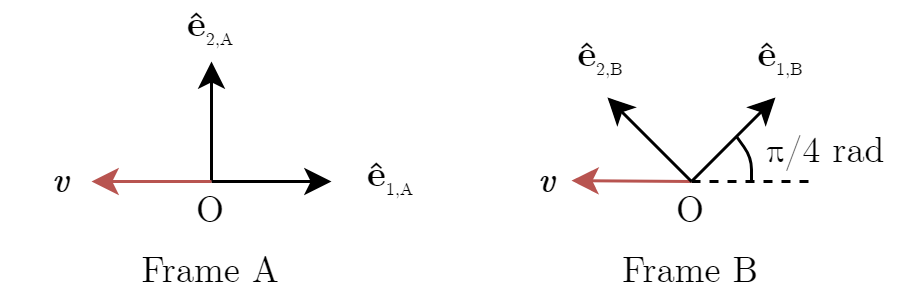
\includegraphics[width=0.75\textwidth]{img/Two_2D_Frames.png}
\end{figure*}

There is also a vector, labeled $\bm{v}$. Looking between the two
frames, we see that $\bm{v}$ isn't moving in space. So the vector
$\bm{v}$ itself is some object in space with a magnitude and direction
that is independent of any reference frames. But the \textit{components} of
$\bm{v}$, which \textit{measure} its magnitude and direction with respect to
some set of basis vectors, \textit{are} dependent on the set of basis vectors.

Consider the components of $\bm{v}$ ``resolved'' in Frame A versus Frame B:
\begin{equation*}
    \bm{v}_A = \begin{bmatrix}
        -1 \\
        0
    \end{bmatrix}
    \quad\quad\quad\quad
    \bm{v}_B = \begin{bmatrix}
        -\cos(\pi/4) \\
        \sin(\pi/4)
    \end{bmatrix}
\end{equation*}

The components of $\bm{v}$ change when resolved (measured) with respect to
different basis vectors (different frames), but the \textit{actual} vector
is stationary in space.

Consider the matrix that rotates Frame A into Frame B (i.e. it rotates the
basis vectors of Frame A by $45^\circ$ anti-clockwise):
\begin{equation*}
    R_{A \to B} = \begin{bmatrix}
        \cos(\pi/4) & -\sin(\pi/4) \\
        \sin(\pi/4) & \cos(\pi/4)
    \end{bmatrix}
\end{equation*}

\textit{However}, applying this matrix to the vector $\bm{v}_A$, we do not
get $\bm{v}_B$:
\begin{equation*}
    \begin{bmatrix}
        \cos(\pi/4) & -\sin(\pi/4) \\
        \sin(\pi/4) & \cos(\pi/4)
    \end{bmatrix}
    \begin{bmatrix}
        -1 \\
        0
    \end{bmatrix}
    =
    \begin{bmatrix}
        -\cos(\pi/4) \\
        -\sin(\pi/4)
    \end{bmatrix}
    \neq
    \bm{v}_B
\end{equation*}

This disparity is because we applied a \textit{rotation} matrix to $\bm{v}_A$,
which one can think of as a function which takes as input the components of
a vector in some reference frame, rotates the vector, and outputs the components
of the rotated vector within that same frame. Effectively, applying
$R_{A \to B}$ to $\bm{v}_A$ is the equivalent of computing

\begin{figure*}[h!]
    \centering
    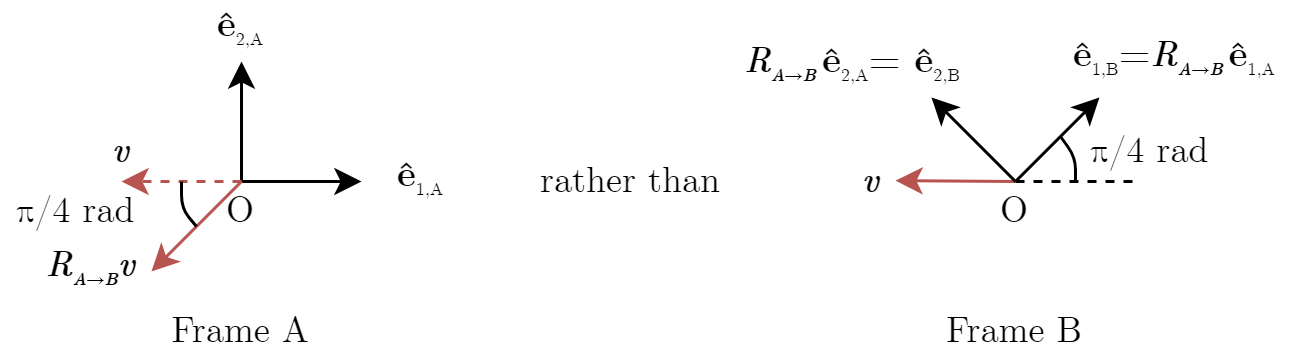
\includegraphics[width=\textwidth]{img/Incorrect Rotation of v.png}
\end{figure*}

You might have noticed, though, that the position of $\bm{v}$ relative to the
basis vectors of Frame B is identical to the position of $\bm{v}$ relative to
the basis vectors of Frame A \textit{had the opposite of $R_{A \to B}$ been
applied to it}. Visually:

\begin{figure*}[h!]
    \centering
    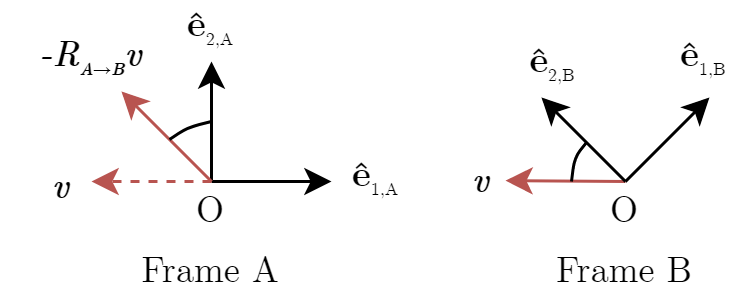
\includegraphics[width=0.75\textwidth]{img/Opposite Relative Rotation.png}
\end{figure*}

Therefore, if we want to find the components of $\bm{v}$ in Frame B, given
its components in Frame A ($\bm{b}_A$) and the rotation matrix from Frame A
to Frame B ($R_{A \to B}$), we must apply the opposite of the rotation matrix:
$\bm{v}_B = -R_{A \to B} \, \bm{v}_A$. However, this notation seems strange,
since we are applying a matrix designed to represent a rotation of a vector
within a frame to a situation in which a vector is not moving in space.
Conventionally, we tend to define a \textit{transformation} matrix which
transforms the components of a vector from one frame to another. In our case,
we can define the matrix $T_A^B = -R_{A \to B}$. The difference in the notation
between rotation and transformation matrix symbols doesn't appear to be
universally used, but it is useful for distinguishing the two when defined.

In summary,
\begin{itemize}
    \item Frames in 2D space require two basis vectors. Conventionally these
          basis vectors are orthonormal.
    \item Vectors are physical objects with a direction and magnitude.
    \item A vector's direction and magnitude can be \textit{measured}
          (or ``resolved'') with respect to the basis vectors of a frame,
          giving numerical values to its components.
    \item In applications where a physical object represented by a vector is
          moving within a single frame (e.g. a robotic arm on a factory line
          moving through a single frame), a rotation matrix aptly describes
          the motion.
    \item In applications where a physical object represented by a vector is
          \textit{not} moving, but rather the engineer wants to know its
          components in with respect to multiple frames, a transformation
          matrix aptly converts the components from one frame to another.
    \item Given the rotation matrix which rotates the basis vectors of one
          frame to another, the transformation matrix which transforms a
          vector's components from the first frame to the second is the
          negative of said rotation matrix.
\end{itemize}